\documentclass{llncs}

\usepackage[a4paper,includeheadfoot,top=1.65in,bottom=1.65in,left=1.73in,hcentering]{geometry}
\usepackage[pdftex]{graphicx}

% Ezek egyikének bekapcsolásával a magyar ékezetes karakterek
% közvetlenül is felhasználhatók:
%\usepackage[latin2]{inputenc} 
\usepackage[utf8]{inputenc}
\usepackage{t1enc}

\usepackage{tikz-dependency}
\usepackage{qtree} % emmegmi? XXX
\usepackage{float}
\restylefloat{figure}
\usepackage{tikz-qtree}

\usepackage[hungarian]{babel}
\selectlanguage{hungarian}

% saját cucc

\usepackage{amsmath}

\usepackage{fullpage} % XXX ezt majd kukázni
\parindent=0pt        % XXX ezt majd kukázni
\parskip=6pt          % XXX ezt majd kukázni

\newcommand{\nyil}{$\rightarrow$\ }
\newcommand{\nnyil}{$\leftrightarrow$\ }
\newcommand{\vnyil}{$\leftarrow$\ }
\newcommand{\code}[1]{\texttt{\small #1}}
\newcommand{\co}[1]{\texttt{\small #1}}
\newcommand{\embf}[1]{\textbf{#1}}
\newcommand{\bd}[1]{\textbf{#1}}
\newcommand{\cc}[1]{\multicolumn{1}{c}{#1}}

\newcommand{\path}[1]{\code{#1}}
\DeclareMathOperator{\distop}{dist}
\newcommand{\dist}[2]{\ensuremath{\distop(\path{#1},\path{#2})}}
%{\sc dist}(\path{#1},\path{#2})}

\newcommand{\liex}[1]{\emph{#1}}

\newcommand{\ittt}{\fbox{\textbf{\_ITT\_T}}\ }

\definecolor{megjcolor}{rgb}{0.50,0.38,0.22} % -- kicsit sötétebb, jobban látszik
\definecolor{alertcolor}{rgb}{1.00,0.40,0.00} % -- durvább ;)
\definecolor{marcicolor}{rgb}{0.20,0.20,1.00} % -- durvább ;)
\newcommand{\XXX}[1]{{\small \color{megjcolor} [XXX #1]}}
\newcommand{\XXXb}[1]{\XXX{\embf{#1}}}
\newcommand{\XXXk}{\XXX{?}\ }
\newcommand{\XXXf}{\XXX{!}\ }
\newcommand{\XXXX}[1]{{\small \color{alertcolor} \bf [XXX #1]}}
\newcommand{\alert}[1]{{\color{alertcolor} \bf #1}}
\newcommand{\marci}[1]{{\color{marcicolor} #1}}

\newcommand{\hmsz}{$\blacktriangleright$} % egy háromszög
\newcommand{\para}[1]{\vspace*{6pt}\hmsz\ \embf{#1}\\}
\newcommand{\cpara}[1]{\vspace*{3pt}{\color{megjcolor}\hmsz\ #1}\\}

\newcommand{\sm}[1]{{\small #1}}
\newcommand{\smp}[1]{{\small (#1)}}
\newcommand{\kov}{\ensuremath{\implies}\ }
\newcommand{\azonos}{\ensuremath{\equiv}\ }
\newcommand{\kb}{\ensuremath{\sim}\ }
\newcommand{\term}[1]{\embf{#1}}

\begin{document}

%\pagestyle{myheadings}
%\def\leftmark{{\rm XIV. Magyar Sz\'am\'\i t\'og\'epes Nyelv\'eszeti Konferencia}}
%\def\rightmark{{\rm Szeged, 2018. január 18-19.}}

%\setcounter{page}{1}

\title{A szöveg mint skálafüggetlen hálózat}
%a november 21-ig bekuldott verziobol kerjuk a szerzok adatait kihagyni
%\author{Makrai Márton és Sass Bálint\\
%  \institute{MTA Nyelvtudományi Intézet\break {\tt \{makrai.marton,sass.balint\}@nytud.mta.hu}}
%}
\author{\institute{}}
\maketitle

% --------------------------------------------------------------------------

\begin{abstract}
Tanulmányunkban a szöveget egy egyszerű konstrukció segítségével
skálafüggetlen hálózatként ábrázoljuk,
és megvizsgáljuk, hogy a hálózatelmélet sztenderd eszközei
mit mondanak \XXXk az ilyen módon reprezentált szövegről.
\\{\bf Kulcsszavak:} hálózatok, skálafüggetlen hálózatok, köztiség, Zipf, gyakoriság, szöveg
\end{abstract}

% --------------------------------------------------------------------------

 
% XXX XXX XXX
% Marci: "Nem annyira zavarja, hogy egyedül csinálja,
%         de hát igen, a cikket meg kéne írni!"
% Marci: "Van olyan eset, hogy poszterre nem fogadják el?" :)
% 
%   + cikk-kezdeményt csinálni -- megvan! :)
%
%   - cikk-kezdeménybe: az ötlet (pár hivatkozással!)
%     ! Marci: "írjam bele az ötletet, mert ha nem sok minden jön ki,
%               akkor a kontribúció jelentős része maga az ötlet lenne!" (!)
%
%   - cikk-kezdeményt közösen szerkeszthetővé tenni
%     ? github? overleaf? (?) XXX :)
%       -- asszem az utóbbi lesz, nincs jobb ötletem :)
%     ! Marci, ne törölj légyszi, semmit se! :)
%
%   - beletenni mindent, ami van :)
%     ! nézzem meg a Marci-féle megosztott doksit
%
%   - kitalálni a további teendőket :)
%
%   - megcsinálni a további teendőket :)
%
%   - beadás előtt: .tex: fullpage-t kukázni! :)

\marci{Ha nem nagy teher, akkor légyszi így írj bele, Marci. :)}


\XXX{nyilván jó lenne 2 bevezető mondat a hálózatelméletről.\\
HIVATK: Barabási-Albert (eredeti cikk), Csermely (közérthető).}

\section{Az ötlet}
% Sztem főként \cite{kovacs2012magyar} alapján...

% Def: sk-f h
Azokat a hálózatokat, ahol a befokszám-eloszlás
Zipf-eloszlást követ, \emph{skálafüggetlen hálózat}oknak nevezzük
\cite[703.\ oldal]{kovacs2012magyar}.
%
A

Befokszám eloszlása Zipf.

Zipf a szöveg.

Ötlet találjunk egy konstrukciót,
amiben a befokszám éppen a szöveggyakoriságot adja.

Így skálafüggetlen hálózatot kapunk.

Az ötlet nagyon egyszerű: ez-és-ez.

% a konstrukció

\begin{figure}[h]
\begin{center}
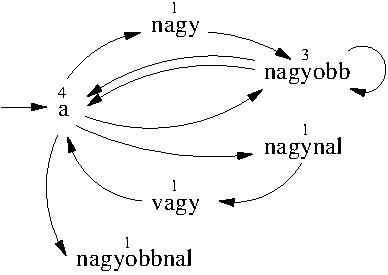
\includegraphics[width=6cm]{scfr_pelda.pdf}
\end{center}
\caption{Példamondatom.
,,a nagyobb nagyobb a nagynál vagy a nagy nagyobb a nagyobbnál''.
A dupla nyilat ábrázolhatjuk egy 2-es súllyal bíró szimpla nyíllal is.
\label{fig:scfr_pelda}}
\end{figure}

És ez nagyon jó, mert így a sk-f hálózatok (hálózatelmélet)
összes meglévő eszközét, módszerét, mérőszámát alkalmazni
tudjuk erre.

Bízunk benne, hogy vmi értelmeset fog mondani ez az eszköztár a szövegről,
hogy vmi értelmes fog kijönni. Lássuk. : )


\section{Vizsgálandó dolgok XXX :)}

\begin{itemize}
\setlength\itemsep{1em}

\item
\embf{erős összefüggőség?}
Az lesz.

2017.11.21. \embf{Marci: erősen (=irányítottan) összefüggő-e a gráf? :)}
Válasz: \embf{hát igen!}
Az \ref{fig:scfr_pelda}.\ ábrán ugye a \emph{nagyobbnál} lóg ki egyedül,
szóval ilyen korpusz elején és végén lévő
különleges szavakból álló ,,farok'' lehet,
ami esetleg nem erősen összefüggő,
de hát biztos minden korpusz \emph{A}-val és ponttal végződik. :)

\item
ugye \embf{kisvilág} a gráfunk?\\
= minden mindenből elérhető mondjuk 6 lépésben
[= legrövidebb utak max hossza 6]\\
\XXXb{Mi a helyzet ezzel?}

\item
\embf{centralitás?}

\begin{itemize}

\item
\emph{[lokális]} \embf{degree centrality} --
Ha ez magas, akkor
,,A csúcspont központi szerepű a lokális környezetében.''
\cite{kovacs2012magyar}.

Jó, ez trivi:
degree centrality \azonos szógyakoriság.
A gyakori szavak azok, amiknek nagy
a degree-centrality-je (befokszám-összege),
és tényleg ők bizonyos értelemben a legfontosabb szavak.

2017.11.21. \embf{Marci:}
,,10 k mondatot nézek.
Odaig jutottam, hogy valóban power law a degree centrality.''
Jó, akkor a kiindulópont megvan (= szöveg szavainak gyakorisága Zi pf). :)
Azaz ez kísérletileg is kijött.

\embf{Ez okés! :) Ez trivi, nem annyira eredmény,
inkább csak ellenőrzés, hogy jó volt-e a kiindulópontunk.}

A \embf{csúcserősség} (esetünkben) tök ugyanez: benyíl-súlyösszeg.

\item
\emph{[globális]} \embf{köztiség (betweenness)}.
Def: (\cite{kovacs2012magyar}-ban sztem zavaros)
sztem: hány legrövidebb út meg át a csomóponton;
avagy: a legrövidebb utak hány \%-a megy át a csomóponton.\\
\XXXb{Mi a helyzet ezzel?}\\
\XXXb{SEJTÉS: olyasmit vélek, hogy ez összefőgg vhogy a szófajokkal,
vagy legalábbis vmilyen típusú szavaknak nagyobb/kisebb lesz.
Pl.\ a névelőnek nem nagy? [Ez már egy bazi jó eredmény lenne sztem!]}

\end{itemize}

\item 
\embf{sűrűség?} 
,,Ha egy hálózati csúcspont néhány lépéses környezetén belüli csúcspontok között viszonylag sok él van, akkor a hálózatnak ezt a tartományát sűrűnek mondjuk.''\\
\XXXb{Mit tudunk mondani a sűrűségről általában? Vagy sűrű tartományokról? Vannak? Hogy is lehet őket megtalálni?}

\item
\embf{$k$-mag?}
Def: $k$-mag = ,,azok a csúcspontok tartoznak ugyanahhoz a $k$-maghoz, amelyek legalább $k$ számú kapcsolattal kötődnek a magban lévő más csúcspontokhoz.''\\
\XXXb{Mit tudunk mondani a $k$-magokról? Hogy találjuk meg őket?}

\item
\embf{csoportok?}
Asszem annyi, hogy belül sűrűek. Csoportszerkezet? (átfedések...)\\
\XXXb{Mit tudunk mondani a csoportokról?
Van a kezünkben csoportkeresési eljárás?
Pl.\ klikk perkolációs algoritmus? (ami magyar találmány elvben)
Átfedhetnek!}

\end{itemize}


\section{Korábbi jegyzetek XXX}

\code{https://github.com/makrai/TextBetweenness} \XXXf

 * ötlet: ,,a szöveg skálafüggetlen hálózat'' -- mondjuk elég trivi ötlet! :)
 -- alapötlet:
    \emph{azért Zipf a szavak, mert vhogyan skálafgtlen hálózatot alkot!}
    \smp{ugye, hogy NEM a szemantikai, szóasszoc, meg hasonló hálózatokkal
         szórakozunk mostan! :)}

 * http://www.greenteapress.com/compmod/html/book006.html
 * https://arxiv.org/pdf/cs/0701135 // 2.2.3 konkrétan :)
 * (Kornai sok Zipf-et ír a matnyelv könyvében, esetleg ezt is említi?)
 \nyil szóval úgy tűnik, hogy ezt már réges rég leírták.
    (azért erre lehetett számítani...)

 \embf{De:} ténylegesen kimondták azt, hogy
 \emph{így (simán közvetlen rákövetkezéssel)
 lehet megkonstruálni a hálózatot, aminek a befokszám összege
 éppen a szógyakoriság lesz, amiről meg (eleve, rég) tudjuk, hogy Zipf,
 azaz skálafüggetlen lesz ez a hálózat
 (éppen mivel a befokszáma Zipf)???} (?!) XXX :)

 -- az itt a nagy eredmény, hogy ez egy skálafüggetlen network lesz, azaz
    minden érvényes lesz rá, ami a skálafüggetlenekre érvényes! (!) XXX :)

 -- de hogy akkor az lenne az "új", hogy erre a hálózatkutatás
    minden eredménye akkor alkalmazható lesz! (!) XXX :)
    -- pl. a "növekedési mechanizmus"-t be lehet mutatni,
       miszerint jön egy új szó, az a növekedési tulajdonság szerint
       illeszkedik be, ez biztosítja, hogy megmarad a skálafüggetlenség! XXX

 \nyil ez nyilván egybecseng a nyelvmodellekkel,
    amik a szavak egymásra következéséről szólnak! (!) XXX :)

 -- szóval ez a két dolog (szavak Zipf \nnyil skálafüggetlen hálózatok)
    akkor oda-vissza szépen megmagyarázza egymást!

 - vö: Varjú Zoli: "Kisvilágunk a nyelv"
   itt (Ferrer és Solé, 2001) eljárását csinálja,
   ami  \emph{nem pont az},  amit én írok!
   \nyil úh esetleg mégis érdekes lehet
      egy MSZNY poszter erejéig megmutatni a gondolatomat! (!) XXX :)
   -- de jó lenne, ha pont az enyémből jönnének olyan szép dolgok,
      ami a Varjú Zoliéból nem, és pont azért, mert
      nem csak a közvetlen rákövetkezést vette! (!) XXX :)

-----

az élsúlyok persze a bigramok, ez trivi.
\smp{az $n$-gramok ($n > 2$) viszont totál nem jelennek meg ebben!}

Viszont a hálózat csomópontjai nem ,,egyneműek'': szófajok vannak.
Ez különleges lehet a sima skálafüggetlen hálózatokhoz képest
(vö: emberek+kutyák hálózata).

A névelőnek sztem nagy lesz a \emph{köztiség (betweenness)} értéke,
és a szófajok talán kijönnek \emph{csoport}okként! :)
\smp{Varjú Zoli mit is ír a funkciószavakról? :)}

\embf{TÖK FONTOS:}
\path{a2a} (\dist{a}{a}=2) nem jelenti azt, hogy van \path{axa} trigram,
csak annyit jelent, hogy van \path{ax} és \path{xa} bigram!
\smp{ez benne az új, izgi! :) [ez is]
-- hm.. bár lehet, h pont ezt tudja
   100 éve trivi módon a sima bigram modell
   \nnyil azért a betweenness meg ezek, hogyzhatnak újat! (!) XXX :)
-- hogy mire lesz jó, azt persze még nem tudom. :)}

-----

Vannak határozott \emph{irányok}
(ti.\ ami csak egyik irányba hajlamos menni), pl.\ névelő \nyil fn.  
Ez nem hat a skálafüggetlenség ellen? Talán nem. (Sztem nem.)

-----

Legrövidebb utak kiszámolása:
nem megy ez a régi concgram-es ,,mindent egyszerre, amit épp tudunk''
ötletem alapján? De sztem megy.
\embf{ld.\ a külön papírkát, ahol bemutatom! -- azt beírni!! :)}\\

Bár biztos van rá 100 más (jobb) módszer... :)

-----

Persze nem csak szavakra megy, hm lemmákra, POS-tagekre, morfémákra.
Hiszen (közismerten) mind Zipf. :) Ezeket is lehet nyomni.

-----

XXX Pollner Péter adna esetleg hozzá szoftvert,
ami alap dolgokat számolgat? :)

XXX többi (esetleg kapcsolódó) megjegyzés 
\cite{kovacs2012magyar} kapcsán: {\tt mk.INFO}.

ilyenek:
-- "szerveződési mintázatok keresése" community detection\\
-- van-e hozzá szoftvercsomag, amivel alap mutatókat lehet számolni?\\
-- további irodalom hozzá

-----

shortest path: gondolkodtam rajta (papírka),
de persze van a Floyd-Warshall algó... :)

-----

toolkit: \embf{NetworKit}
linkgroup (Csermely Péter) / links / Network analysis
-- Get started + NetworKit User Guide, \emph{kipróbálni nagyon!}

2017.11.08. vagy esetleg épp Neo4j -vel lenne érdemes csinálni? :)
% https://db-engines.com/en/article/Graph+DBMS

2017.11.14. Vedres Balázs: "az elemzést Matlab-ban végeztem,
csak az alap mátrixaritmetikai funkciókkal. A NetworKit-et nem ismerem."
-- hú és akkor hogy számolt betweenness-t, meg klikk-perkolációt, stb-t? :)


-----

ACL Anthology: search: scale-free, NetworKit
\nyil foglalkozott ezzel bárki?\\
\embf{"scale-free" bigram} \nyil 20 találat, ezeket végig kell nézni! XXX :)\\
\embf{"scale-free" bigram betweenness} \nyil 3 találat, ezeket még inkább! XXX :)

-----

ez a scale-free bigramos modell tökre segíthet kitalálni a pázmányos
elemző dolgait! :) merthogy pont a rákövetkezési szabályokról mond vmit! :)

-----

persze a "2-vel utána következő szó"-ból is scale-free network jön ki
(lényegében tuti, de azért ellenőrizzem),
aminek első ránézésre nem sok teteje van, de ki tudja... :)

-----

CEU Center for Network Science -- Vedres Balázs, Kertész János

-----

azzal, hogy a sorrend nálam nagyon számít
(vö: \cite{kovacs2012magyar} simán szimmetrikus ablakot vett)
\emph{szemantikus} helyett \emph{szintaktikus} hálózatot kapunk
= reményem szerint kijönnek a szófajok.

-----

meetup Berend Gáborról:
,,he also has a keen interest in network science'' (!) :)


% --------------------------------------------------------------------------


%%%% XXX XXX XXX XXX XXX a végsőbe ez nagyon kell! (!) XXX XXX XXX XXX XXX
%%%% \section*{Köszönetnyilvánítás}
%%%% \label{Koszonet}
%%%% 
%%%% XXX Sass Bálint kutatásait az MTA Bolyai János ösztöndíja támogatta.

% ---- Bibliography ----
%
%kulon bibtex fajl hasznalata
\bibliographystyle{splncs}
\bibliography{minden.bib}

\end{document}
